\section{Results}
\label{sec:results}

The results are separated by gas, but not by monitoring station. We present
more detailed results for only one (Tijuca station was chosen randomly), and after aggregated results
considering all the stations. This is done because we have more than
a hundred models to analyse. To deal with this diversity, the steps
(hyperparameters choice and evaluation) are automated. We are
making predictions one hour ahead and it is possible to compare with one day
ahead models. After this, we will have a best model for each gas and each
station (23 on total). 

\subsection{Tijuca monitoring station}

The results follow the order specified in the above summary for each pollutant. 

\subsubsection{Ozone}

{\em Simple linear regression}

\vspace{2mm}

Applying simple linear regression, the $R^2$ in the testing set was 0.837,
which appears to be a good start fitting. The variable with greater t-statistic
was O$_3$ shifted by one hour. Other features with great t-statistic (more than
20) was, in
order, wind speedy, ozone lag 2, hour sin, UR, ozone lag 24, hour cos, and RS.
This is interesting because we have already observed the hourly seasonality
and by the formation of ozone, RS is expected to influence (not necessarily
linearly). The shifts were expected by the autocorrelation graph. Only some few features (3) had p-value greater that 0.05. The
F-statistic considering all variables was practically zero. One important
problem with this approach was the very big condition number (3.4e+06) given
the observed multicollinearity. Figure \ref{fig:histogram-residuals-slr} shows
that the histogram of the residuals is very similar to a normal distribution (as
assumed by the model).The kurtosis was nearly 3, while the skewness around
0.22. Jarque-Bera rejects the null hypotheses that skewness and kurtosis are the same
as normal distribution, though. The fitting result in testing data can be
partially observed in Figure \ref{fig:observed-fitting-ozone-tijuca}. Looking
at Figure  \ref{fig:observed-vs-residual-linear-regression}, as larger the
observed ozone gets, the more underestimated the prediction is.

\begin{figure}
    \centering
    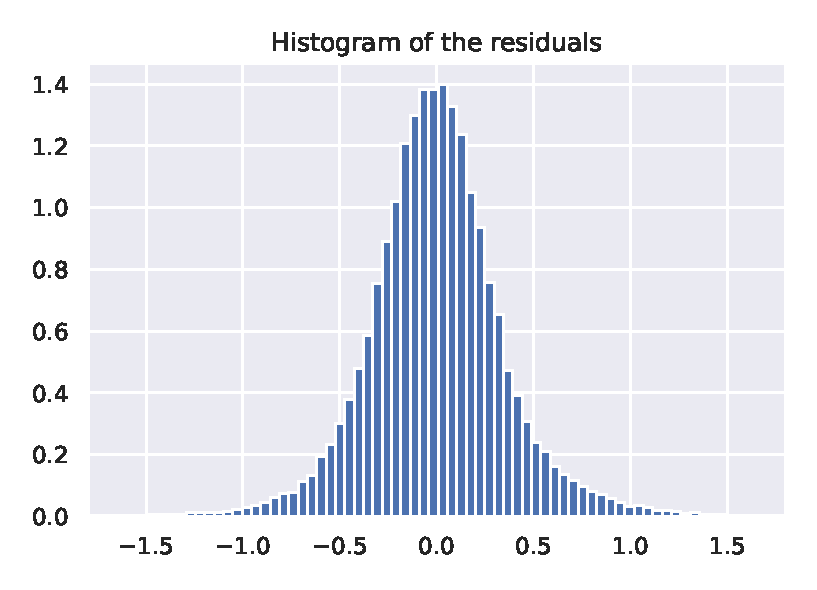
\includegraphics[width=0.45\textwidth]{histogram_residuals_slr.eps}
    \caption{Histogram of the residuals of simple linear regression model for ozone.}
    \label{fig:histogram-residuals-slr}
\end{figure}

\begin{figure}[!ht]
    \centering
    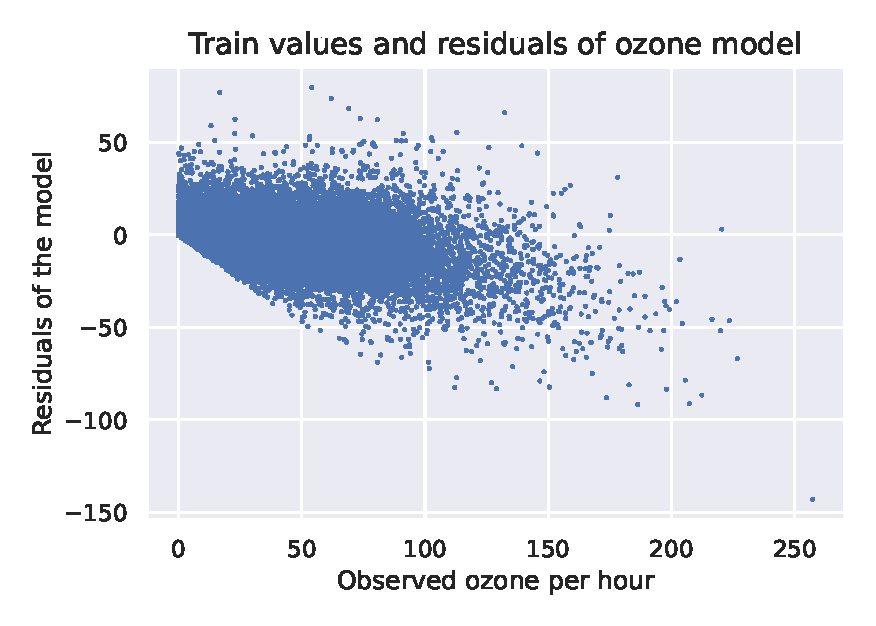
\includegraphics[width=0.45\textwidth]{observed-vs-residuals-linear-regression.eps}
    \caption{Simple linear regression residuals plotted against
    observed ozone values.}
    \label{fig:observed-vs-residual-linear-regression}
\end{figure}

When the lags 1 and 2 are removed, that is, only using the lag 24, the metrics
get much worse. In special, $R^2$ is around 0.49. Figure \ref{fig:r2-test-lag}
presents how the linear models performs badly when the first lags are removed.

\begin{figure}[!ht]
    \centering
    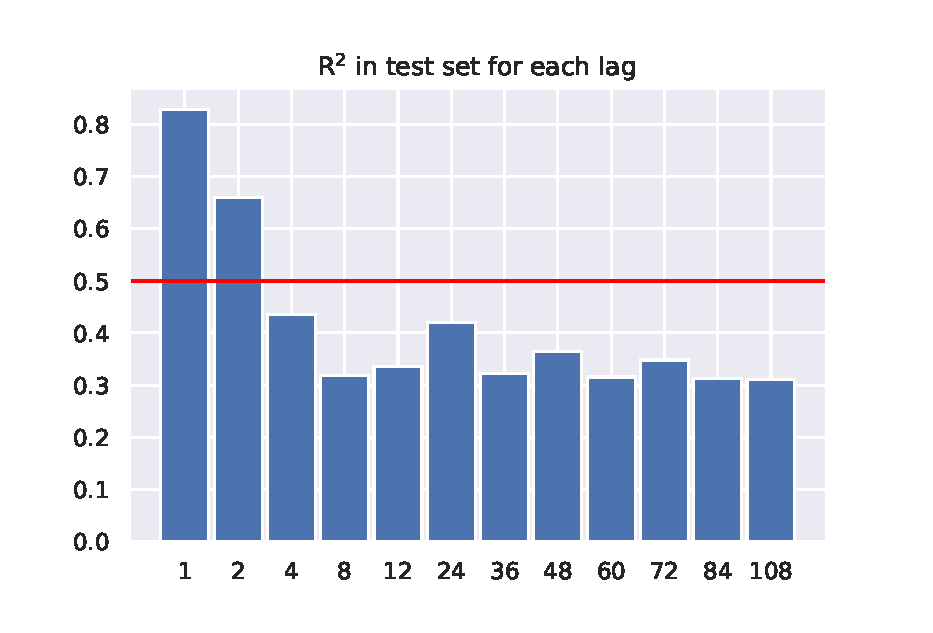
\includegraphics[width=0.45\textwidth]{r2_test_per_lag.eps}
    \caption{Removing all lag variables, adding only one per time, and calculating the R$^2$ in the test set.}
    \label{fig:r2-test-lag}
\end{figure}

\begin{figure*}[!ht]
    \centering
    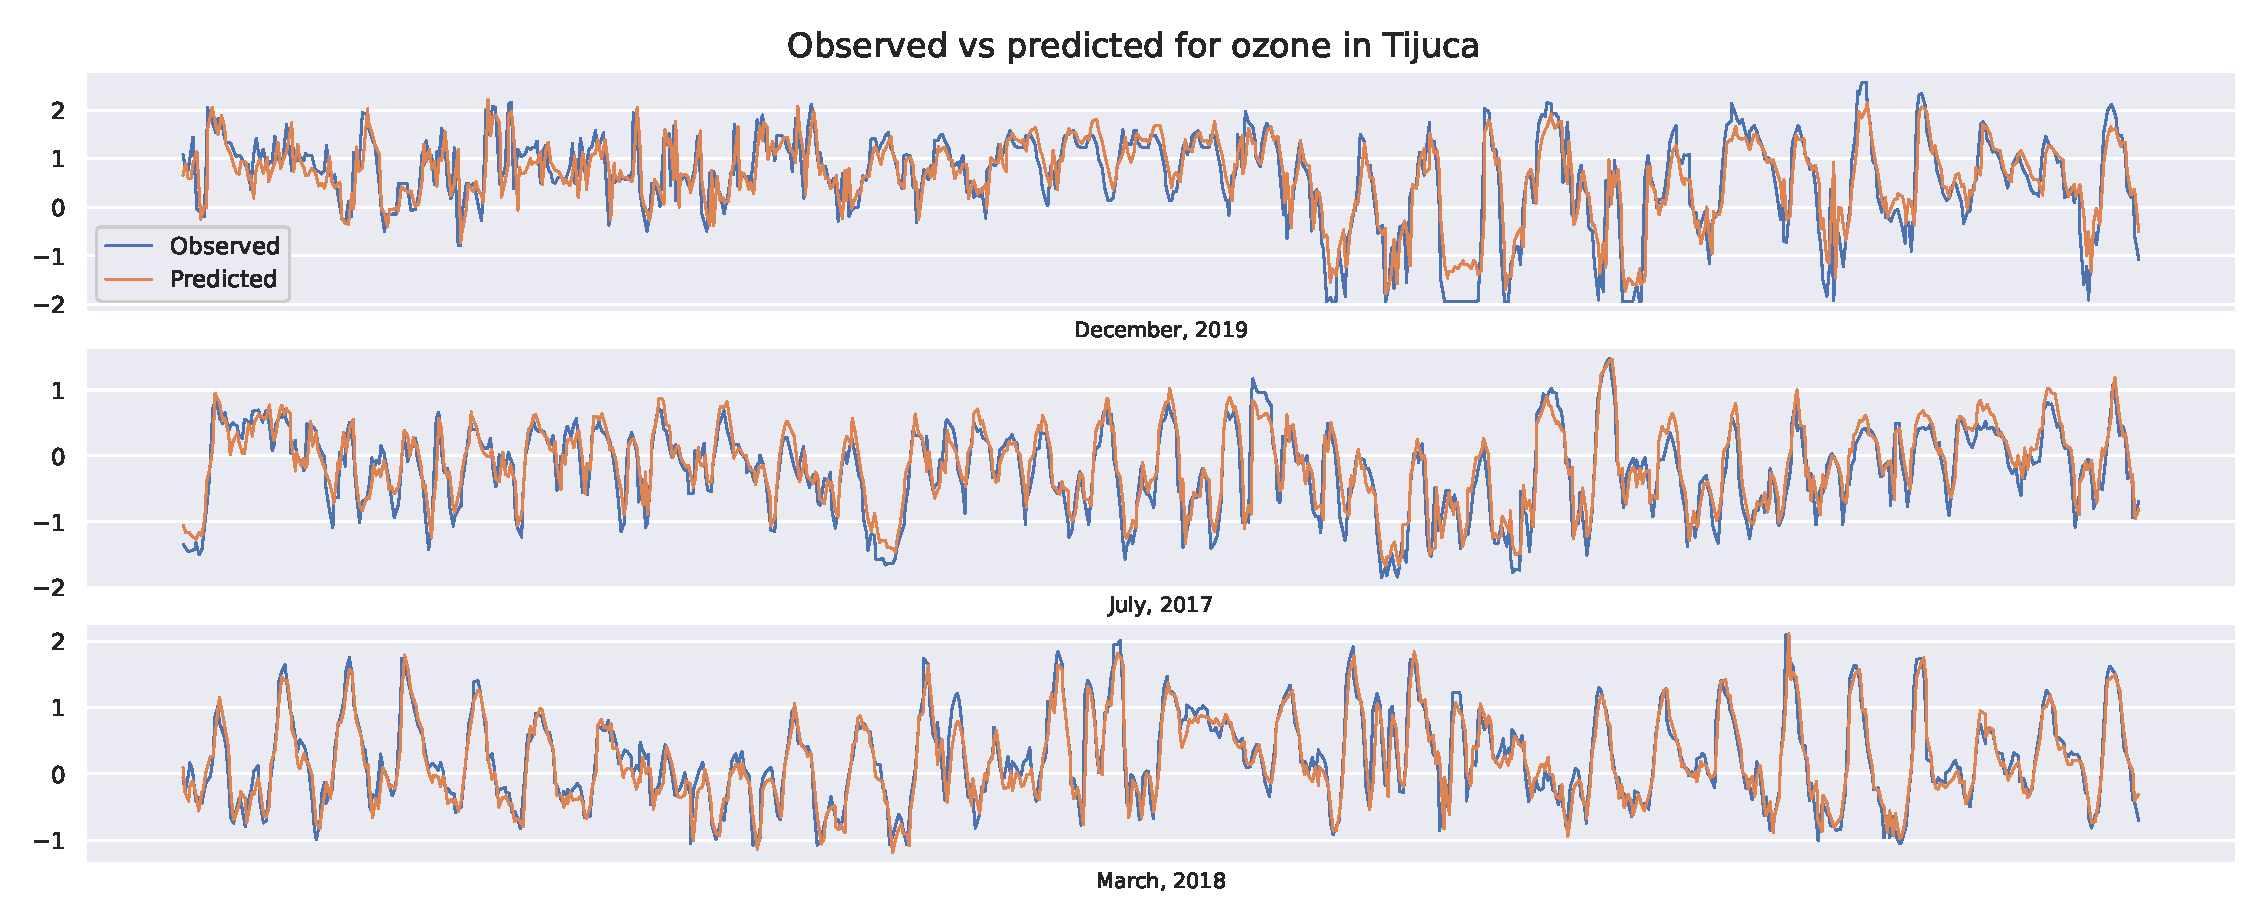
\includegraphics[width=\textwidth]{observed-fitting-ozone-tijuca.eps}
    \caption{Observed and predicted ozone values for different months in Tijuca.}
    \label{fig:observed-fitting-ozone-tijuca}
\end{figure*}

\vspace{2mm}

{\em Elastic-net regression}

\vspace{2mm}

One important observation is that the interaction terms make the metrics worse
in simple linear regression and are disregarded for that reason. In this
case, they improve a lot. There are 376 features considering the polynomial
and interactions. The hyperparameters were set to $\alpha = 2$ and
$w_{l1} = 0.9$, what force several parameters to be zero. Only 6\% of the
variables ended to be non null. All the non zero coefficients were related to interactions with the {\tt year} variable.
This is related to Figure \ref{fig:time-series-gases-year}. $R^2$ in the test
set was 0.838, a few more than the simple linear regression. The histogram of
the residuals are similar to Figure \ref{fig:histogram-residuals-slr}, and
skewness and kurtosis too.

\begin{remark}
    Without interaction terms, the $R^2$ was around 0.5 and $\alpha$ was
    almost 0. 
\end{remark}

\vspace{2mm}

{\em Feature selection + Linear regression}

\vspace{2mm}

Feature selection was performed (proper code) with 5-Fold cross validation and
threshold equals to 0.001, that is, if the $R^2$ score improves less than
0.001, the features stop to be added in the best subset. The chosen features
were {\tt year * O3\_lag1}, {\tt RS}, {\tt RS * hour\_cos}, {\tt year *
Vel\_Vento}, {\tt O3\_lag2}, {\tt year O3\_MA24}, {\tt hour\_cos \* PM10\_lag1},
{\tt RS * Temp}, {\tt RS * O3\_lag2}, and {\tt O3\_lag1**2}. Note that it is
very different from those selected by elastic net. All the variables had
p-value less than 0.001, histogram similar to
\ref{fig:histogram-residuals-slr}, and Jarque-Bera indicating non-normality.
The $R^2$ in testing data was 0.848. 

Other important consideration is that the condition number is still big:
9.72e+03, despite being smaller than in simple regression case. After
calculating the Pearson correlation between the best variables, {\tt O3\_lag2}
and {\tt year * O3\_lag1} have more than 0.8, what was expected and even used.
Some experiments were conducted to reduce this value, but none was successful.
It appears that all variables are strongly (and linearly) related but also
add some information to prediction (at least a subset of them). This is bad
for the interpretation of the coefficients, since its identifiability cannot
be proved.  

\begin{remark}
    Solar radiation had a positive coefficient, so when it increases one unit
    of standard deviation, the ozone grows too. 
\end{remark}

\vspace{2mm}

{\em Support Vector Regression}

\vspace{2mm}

We remember that this model is computationally very costly, so its optimality
is not reached. From the cross validation, the best hyperparameters were
$\epsilon = 0.2$ and $C = 1.0$. With these values, we perform the linear SVR and
the SVR with kernel RBF only to compare them (it is practically
impossible to handle this amount of data with grid search when RBF kernel is
used in only one computer).

Setting those parameters, SVR with kernel RBF took 6min 28s (CPU time), while
Linear SVR 13.1s (CPU time). With RBF kernel, the $R^2$ in testing data was 0.78 and
with linear, it was 0.839. Looking at $R^2$ in training data, we observe that
the non-linear kernel suffered with over-fitting. Residues have not changed
much from the latest graphs, neither kurtosis nor skewness.

Considering the dataset with polynomial and interaction terms, we used the
best features chosen by Forward Feature Selection in the linear regression case. The
$R^2$ in testing data grew to 0.848 (the same as in the linear regression
case). The hyperparameters were not changed. Feature selection could be done with this model too, but it would be
too costly. Finally, the SVR with RBF kernel was performed with the best
features. The $R^2$ in testing set was 0.851. 

\vspace{2mm}

{\em Random Forest} 

\vspace{2mm}

This algorithm is also very costly for large datasets, specially caused by the
choice of $s$ or other parameters, such as, max depth. This makes it harder to
do grid search to choose the best parameters. First, we consider that $s \in
\{10, 20, 50, 100\}$, $c \in \{0.0, 0.0001, 0.001, 0.01, 0.1, 1\}$, and $B =
100$. The chosen parameters were $s = 10$ and $c = 0$ (no regularization).
With this setting, $R^2$ in testing set was 0.848. From this result, we change
the the grid search to $s \in
\{2, 5, 8\}$ and $c \in \{0.0, 0.01, 1\}$. As expected, the selected were $c =
0.0$ and $s = 2$. However, despite needing more time, the $R^2$ in the testing
set did not improve. 

\vspace{2mm}

{\em Linear regression with missing data} 

\vspace{2mm}

The first thing we should note is that the parameters are different from
the linear regression with fixed imputation, but not so much. The ratio
between the estimated parameters ranged according to Figure
\ref{fig:boxplot-linear-regression}. 

The $R^2$ in the testing set was 0.84, a little better than in the simple
linear regression case. Considering the best features with polynomial and
interactions terms, the $R^2$ was 0.847.

\begin{figure}
    \centering
    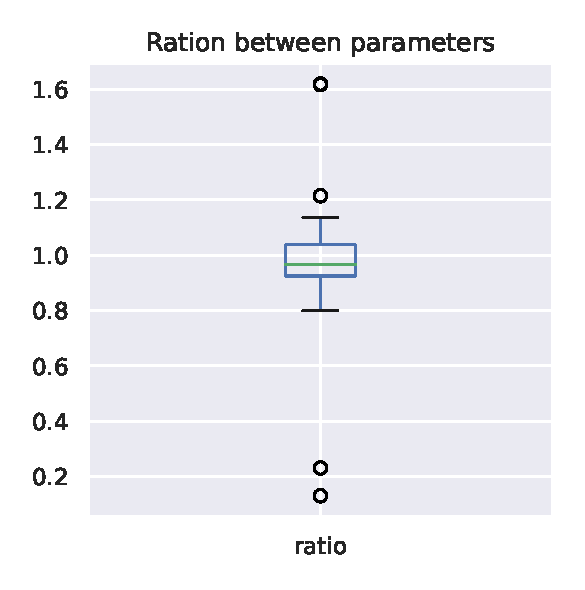
\includegraphics[width = 0.4\textwidth]{boxplot_ratio_linear_regression.eps}
    \caption{Boxplot with the ratios of the parameters from linear regression
    with imputation for the parameters with no imputation.}
    \label{fig:boxplot-linear-regression}
\end{figure}

\vspace{2mm}

{\em Model comparison} 

\vspace{2mm}

The best model was the Random Forest with the best features (selected by linear model) regarding the three metrics. Figure
\ref{fig:model-comparison-ozone-tijuca} presents the results for RMSE. Observe
the range in y axis goes from 0.2 to 0.36 to emphasize the difference.

\begin{figure}
    \centering
    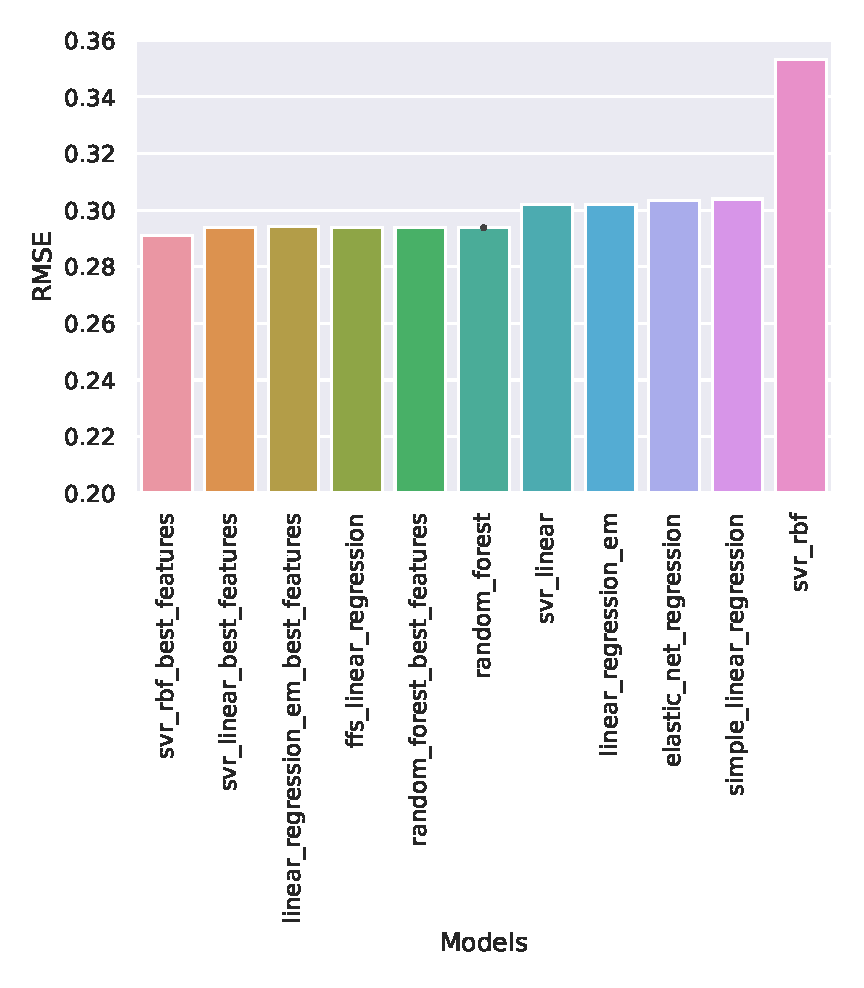
\includegraphics[width = 0.4\textwidth]{model-comparison-ozone-tijuca.eps}
    \caption{Comparison among the models for ozone concentration at Tijuca monitoring station.}
    \label{fig:model-comparison-ozone-tijuca}
\end{figure}

\subsubsection{Carbon monoxide}

{\em Simple linear regression}

\vspace{2mm}

With the linear regression, the $R^2$ in the testing set was 0.849,
what is pretty good when compared to the results from the ozone model. The variable with greater t-statistic
was CO shifted by one hour, what was already expected. Other features with
large t-statistic (absolute value more than
20) was, in
order, hour cos, wind speedy (again!), CO with 24 moving average, O3 with lag
1, CO with lag
2, and hour sin. Besides the hourly seasonality and wind speed, all the
variables are related to the gases. This may be related to the fact that CO is
produced by combustion and car traffic. Only some few features (3) had p-value
greater that 0.05. The F-statistic considering all variables was practically zero. Figure \ref{fig:histogram-residuals-co-slr} shows
the histogram of the residuals very similar to a normal distribution (as
assumed by the model).The kurtosis was greater than 4, while the skewness around
-0.3. Jarque-Bera corroborates with the non-normality. The fitting result in testing data can be
partially observed in Figure \ref{fig:observed-fitting-co-tijuca}.  Figure
\ref{fig:observed-vs-residual-co-linear-regression} has the same behavior as
the model for ozone.  

\begin{figure}
    \centering
    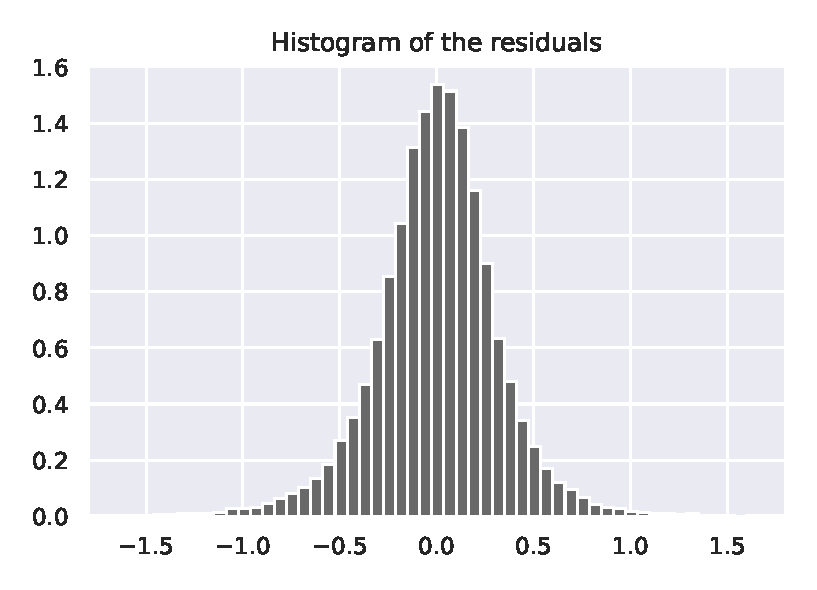
\includegraphics[width=0.45\textwidth]{histogram_residuals_co_slr.eps}
    \caption{Histogram of the residuals of simple linear regression model for CO.}
    \label{fig:histogram-residuals-co-slr}
\end{figure}

\begin{figure}[!ht]
    \centering
    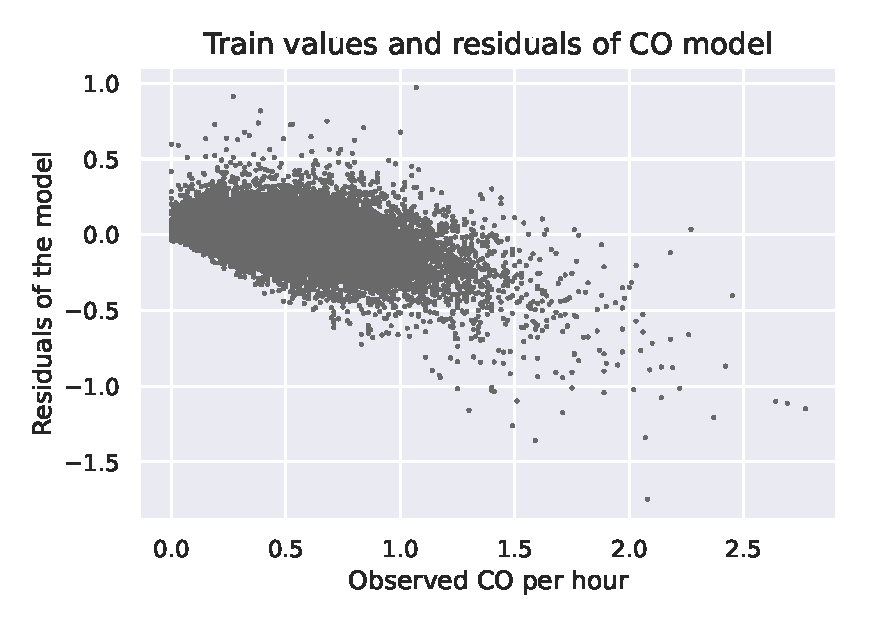
\includegraphics[width=0.45\textwidth]{observed-vs-residuals-co-linear-regression.eps}
    \caption{Simple linear regression residuals plotted against
    observed CO values.}
    \label{fig:observed-vs-residual-co-linear-regression}
\end{figure}

Figure \ref{fig:r2-test-lag-co} presents how the linear models performs badly when the first lags are removed.

\begin{figure}[!ht]
    \centering
    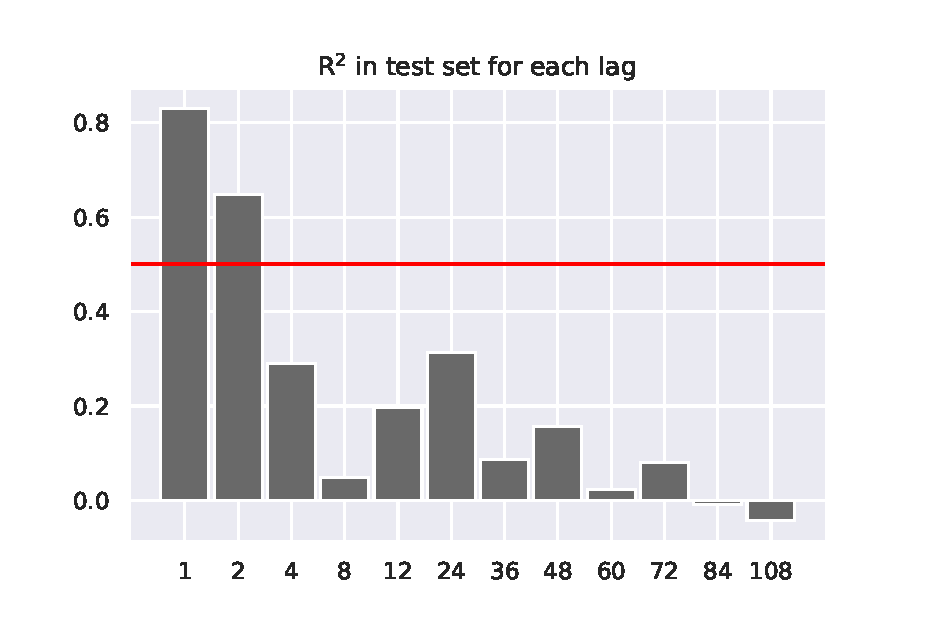
\includegraphics[width=0.45\textwidth]{r2_test_per_lag_co.eps}
    \caption{Removing all lag variables, adding only one per time, and calculating the R$^2$ in the test set.}
    \label{fig:r2-test-lag-co}
\end{figure}

\begin{figure*}[!ht]
    \centering
    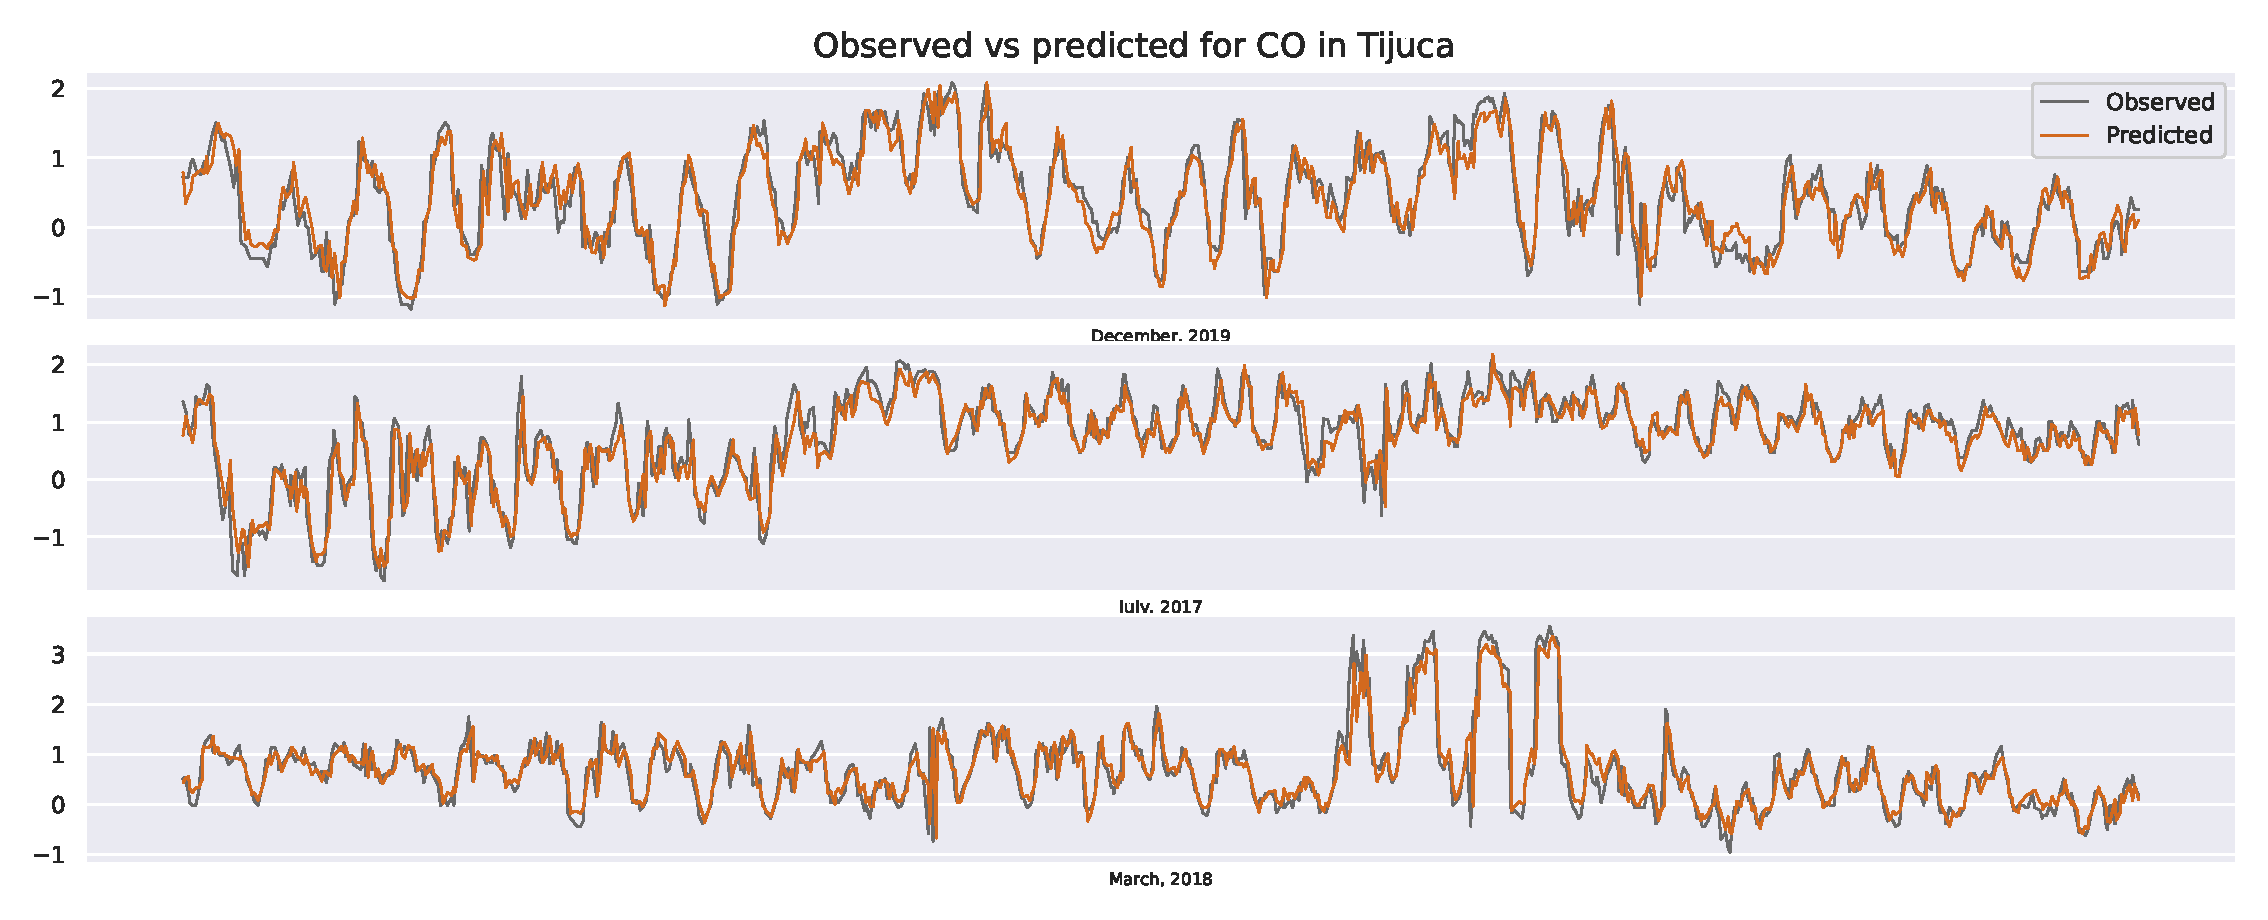
\includegraphics[width=\textwidth]{observed-fitting-co-tijuca.eps}
    \caption{Observed and predicted CO values for different months in Tijuca.}
    \label{fig:observed-fitting-co-tijuca}
\end{figure*}

\vspace{2mm}

{\em Elastic-net regression}

\vspace{2mm}

Differently from the ozone model, the hyperparameters were set to $\alpha = 1$
and $w_{l1} = 0.1$, what forces the $\mathcal{L}_2$ penalty and reduces
variability. Only 7\% of the variables ended to be non null. The result was interesting because all the non
zero coefficients were related to interactions with the {\tt year} variable.
This is related to Figure \ref{fig:time-series-gases-year}. $R^2$ in the test
set was 0.849, very similar to the simple linear regression. 

\vspace{2mm}

{\em Feature selection + Linear regression}

\vspace{2mm}

The chosen features for this model by forward feature selection were {\tt CO\_lag1}, {\tt hour\_sin**2},
{\tt CO\_lag24}, {\tt hour\_cos}, {\tt year Vel\_Vento}, {\tt CO\_MA24}, {\tt RS PM10\_lag1}, {\tt CO\_lag2}, and {\tt Vel\_Vento**2}. Note that it is
very different from those selected by elastic net. All the variables had
p-value less than 0.001, histogram similar to
\ref{fig:histogram-residuals-slr}, and Jarque-Bera indicating non-normality.
The $R^2$ in testing data was 0.852. Here the condition number was still large
and to preserve predictability, it has been left out. 

\begin{remark}
    The sine of the hour had a positive coefficient, while the cosine a
    negative one. 
\end{remark}

\vspace{2mm}

{\em Support Vector Regression}

\vspace{2mm}

From the cross validation, the best hyperparameters were
$\epsilon = 0.2$ and $C = 0.1$. With these values, we perform the linear SVR and
the SVR with kernel RBF. SVR with kernel RBF took 1min 17s (CPU time), while Linear SVR 0.35s (CPU time). With RBF kernel, the $R^2$ in testing data was 0.767 and
with linear, it was 0.848. Residues have not changed
much from the latest graphs, neither kurtosis nor skewness.

Considering the dataset with polynomial and interaction terms, we used the
best features chosen by Forward Feature Selection in the linear regression case. The
$R^2$ in testing data grew to 0.852. Feature selection could be done with this model too, but it would be
too costly. Finally, the SVR with RBF kernel was performed with the best
features. The $R^2$ in testing set was 0.838. 

\vspace{2mm}

{\em Random Forest} 

\vspace{2mm}

The chosen parameters were $s = 20$ and $c = 0$ (no regularization).
With this setting, $R^2$ in testing set was 0.848. From this result, we change
the the grid search to $s \in
\{2, 5, 8\}$ and $c \in \{0.0, 0.01, 1\}$. The selected were $c =
0.0$ and $s = 5$, with a little lower cross validation score. Considering
polynomial terms and the best features, the result was 0.852. 

\vspace{2mm}

{\em Linear regression with missing data} 

\vspace{2mm}

The ratio between the estimated parameters ranged according to Figure
\ref{fig:boxplot-co-linear-regression}, showing a similar estimation in most cases. The $R^2$ in the testing set was
0.849, same as in the simple
linear regression case. Considering the best features with polynomial and
interactions terms, the $R^2$ was 0.852. 

\begin{figure}
    \centering
    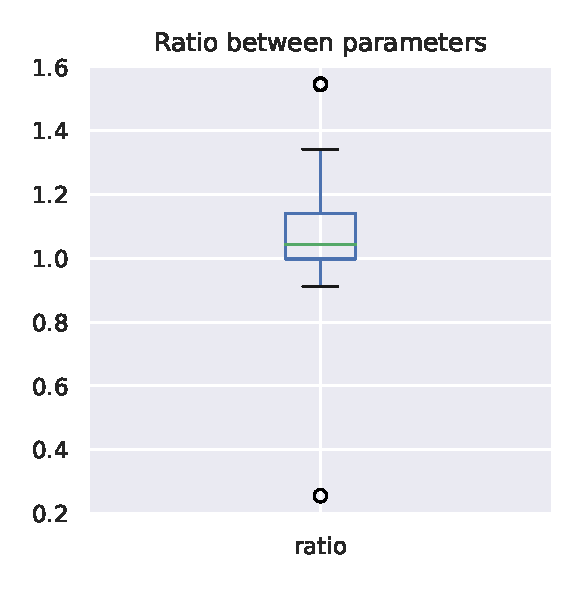
\includegraphics[width = 0.4\textwidth]{boxplot_ratio_co_linear_regression.eps}
    \caption{Boxplot with the ratios of the parameters from linear regression
    with imputation for the parameters with no imputation.}
    \label{fig:boxplot-co-linear-regression}
\end{figure}

\vspace{2mm}

\vspace{2mm}

{\em Model comparison} 

\vspace{2mm}

The best model was the SVR with RBF kernel and the best features
(selected by linear model) regarding the three metrics. Figure
\ref{fig:model-comparison-co-tijuca} presents the results for RMSE. Observe
the range in y axis goes from 0.2 to 0.36 to emphasize the difference.

\begin{figure}
    \centering
    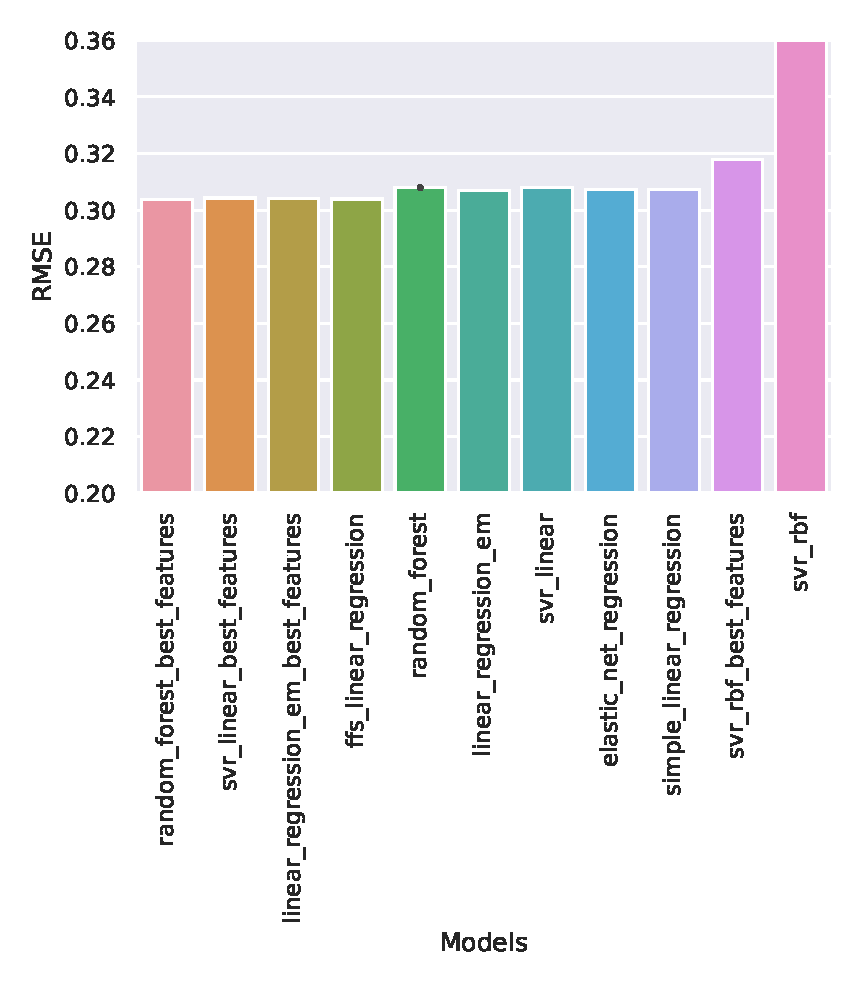
\includegraphics[width = 0.4\textwidth]{model-comparison-co-tijuca.eps}
    \caption{Comparison among the models for CO concentration at Tijuca monitoring station.}
    \label{fig:model-comparison-co-tijuca}
\end{figure}


\subsubsection{Particulate matter 10}

{\em Simple linear regression}

\vspace{2mm}

The $R^2$ in the testing set was 0.8, worse than the previous gases. The
variable with greater t-statistic was PM$_{10}$ shifted by one hour, what was already expected. Other features with
large t-statistic (absolute value more than
20) was, in
order, CO lag 1, PM$_{10}$ with 24 moving average, CO with lag
2, and O$_{3}$ lag 1. This indicates that the model is very poor when only
using the meteorological variables. 7 features had p-value
greater that 0.05, a lot when compared to the previous models. The F-statistic considering all variables was practically zero. Figure \ref{fig:histogram-residuals-pm10-slr} shows
the histogram of the residuals very similar to a normal distribution (as
assumed by the model).The kurtosis was greater than 3, while the skewness around
-0.05. Despite the similarity to the normal distribution, Jarque-Bera rejects
it. The fitting result in testing data can be
partially observed in Figure \ref{fig:observed-fitting-pm10-tijuca}.  Figure
\ref{fig:observed-vs-residual-pm10-linear-regression} has the same behavior as
the model for ozone.  

\begin{figure}
    \centering
    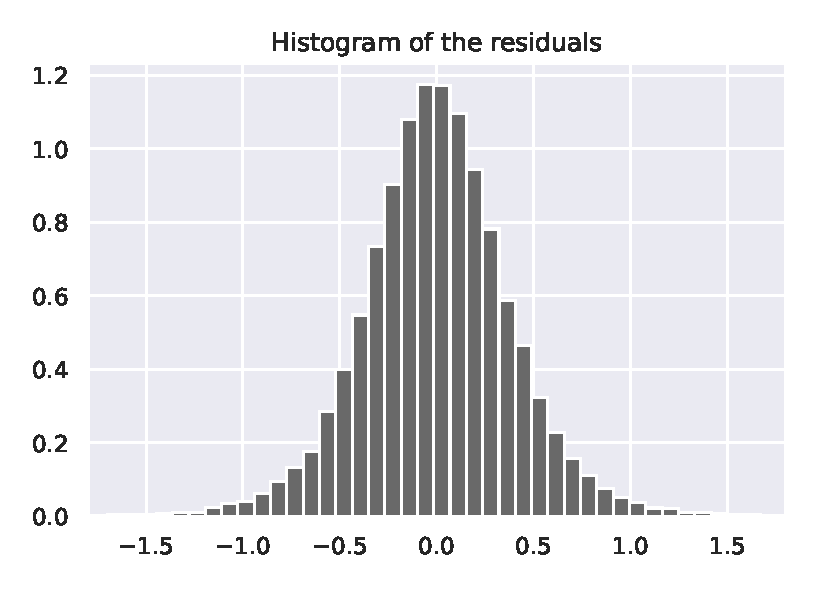
\includegraphics[width=0.45\textwidth]{histogram_residuals_pm10_slr.eps}
    \caption{Histogram of the residuals of simple linear regression model for PM$_{10}$.}
    \label{fig:histogram-residuals-pm10-slr}
\end{figure}

\begin{figure}[!ht]
    \centering
    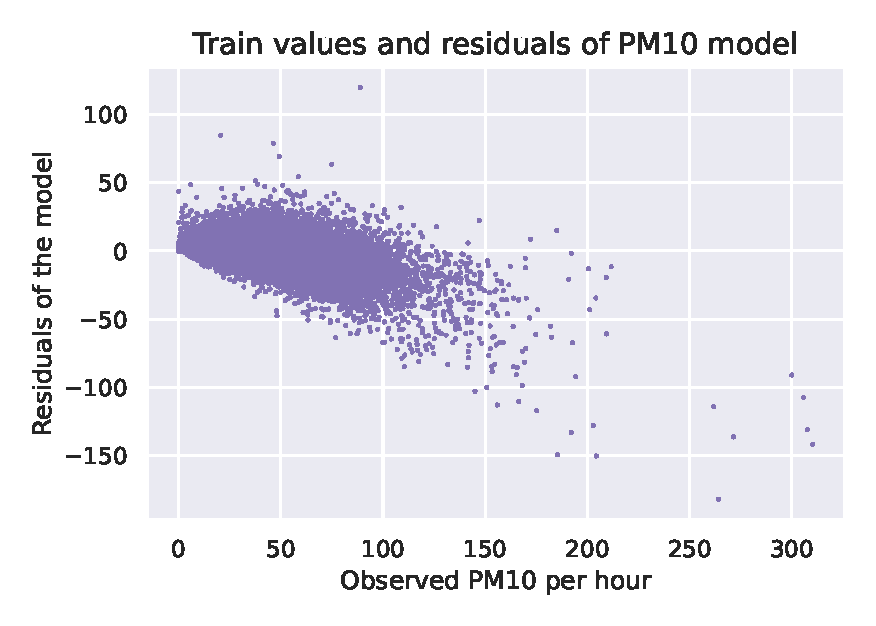
\includegraphics[width=0.45\textwidth]{observed-vs-residuals-pm10-linear-regression.eps}
    \caption{Simple linear regression residuals plotted against
    observed PM$_{10}$ values.}
    \label{fig:observed-vs-residual-pm10-linear-regression}
\end{figure}

\begin{figure*}[!ht]
    \centering
    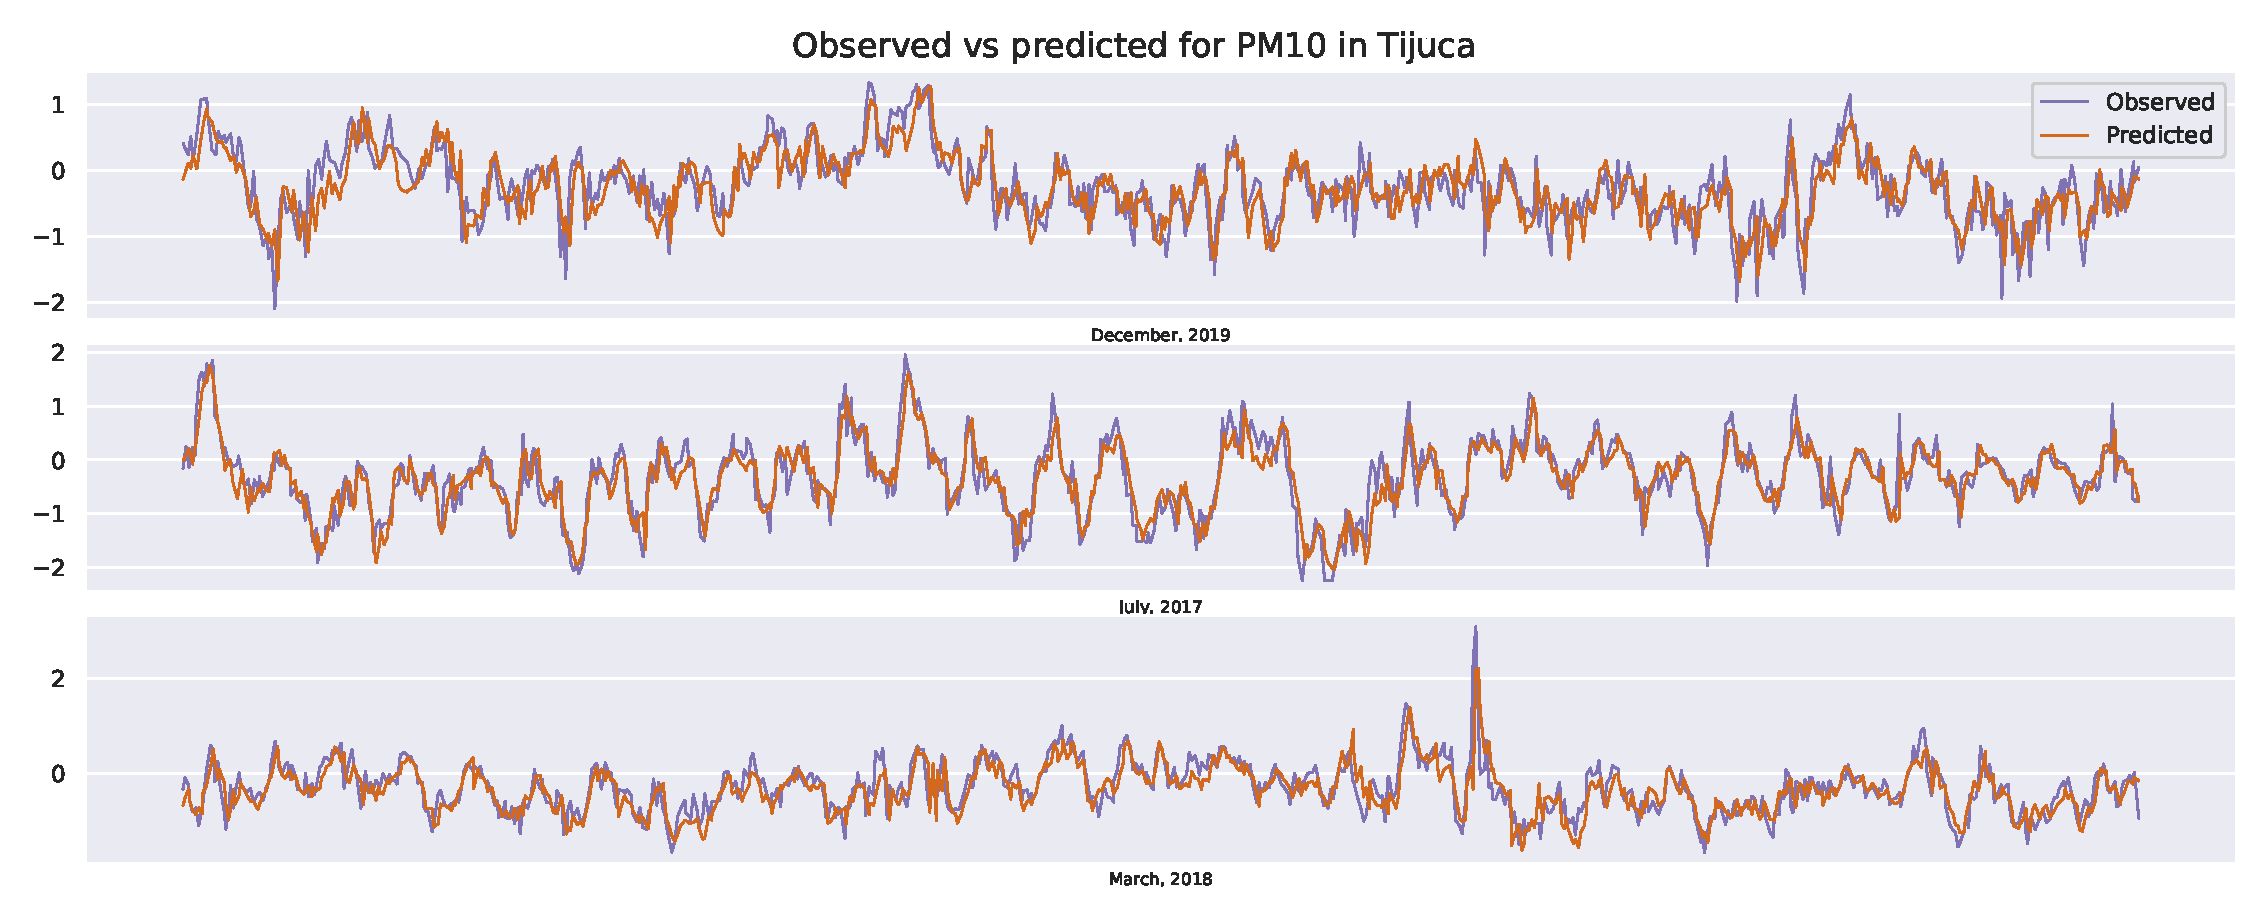
\includegraphics[width=\textwidth]{observed-fitting-pm10-tijuca.eps}
    \caption{Observed and predicted PM$_{10}$ values for different months in Tijuca.}
    \label{fig:observed-fitting-pm10-tijuca}
\end{figure*}

\vspace{2mm}

{\em Elastic-net regression}

\vspace{2mm}

The hyperparameters were set to $\alpha = 3$
and $w_{l1} = 1$, that is only $\mathcal{L}_1$ penalty. Only 5.8\% of the
variables ended to be non null, and all were related to interactions with
year. $R^2$ in the test set was 0.797.

\vspace{2mm}

{\em Feature selection + Linear regression}

\vspace{2mm}

The chosen features for this model by forward selection were {\tt
PM10\_lag1}, {\tt year PM10\_MA24},
{\tt hour\_cos}, {\tt O3\_lag1}, {\tt year O3\_lag2}, {\tt CO\_MA24}, {\tt
hour\_sim hour\_cos}, {\tt year Temp}, {\tt RS O3\_lag2}\ and {\tt O3\_lag**2}
. All the variables had p-value less than 0.001, histogram similar to
\ref{fig:histogram-residuals-pm10-slr}, and Jarque-Bera indicating non-normality.
The $R^2$ in testing data was 0.79, worst then above.

\vspace{2mm}

{\em Support Vector Regression}

\vspace{2mm}

From the cross validation, the best hyperparameters were
$\epsilon = 0.01$ and $C = 0.1$. With these values, we perform the linear SVR and
the SVR with kernel RBF. SVR with kernel RBF took 2min 52s (CPU time), while Linear SVR 1.52s (CPU time). With RBF kernel, the $R^2$ in testing data was 0.783 and
with linear, it was 0.8. Residues have not changed much from the latest graphs, neither kurtosis nor skewness.

Considering the dataset with polynomial and interaction terms, we used the
best features chosen by Forward Feature Selection in the linear regression case. The
$R^2$ in testing data grew to 0.793. SVR with RBF kernel got worse to 0.798. 

\vspace{2mm}

{\em Random Forest} 

\vspace{2mm}

The chosen parameters were $s = 10$ and $c = 0$ (no regularization).
With this setting, $R^2$ in testing set was 0.803. From this result, we change
the the grid search to $s \in
\{2, 5, 8\}$ and $c \in \{0.0, 0.01, 1\}$. The selected were $c =
0.0$ and $s = 5$, with the same cross validation score. Considering
polynomial terms and the best features, the result was 0.791. 

\vspace{2mm}

{\em Linear regression with missing data} 

\vspace{2mm}

The $R^2$ in the testing set was 0.794 and with the best features from
polynomial and interactions terms, the $R^2$ was 0.79.

{\em Model comparison} 

\vspace{2mm}

The best model was random forest regarding the three metrics. Figure
\ref{fig:model-comparison-pm10-tijuca} presents the results for RMSE. Observe
the range in y axis goes from 0.2 to 0.4 to emphasize the difference.

\begin{figure}
    \centering
    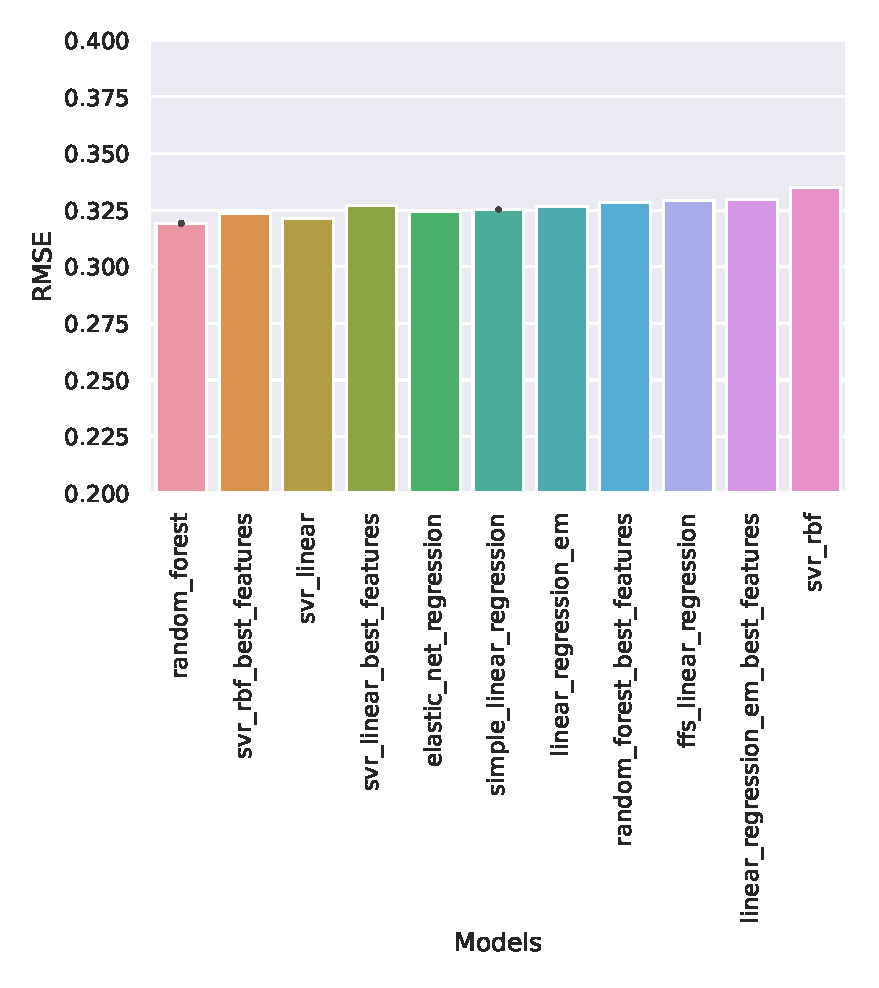
\includegraphics[width = 0.4\textwidth]{model-comparison-pm10-tijuca.eps}
    \caption{Comparison among the models for PM$_{10}$ concentration at Tijuca monitoring station.}
    \label{fig:model-comparison-pm10-tijuca}
\end{figure}

\subsubsection{Air quality index prediction}

In order to predict AQI, we use the best model for each pollutant
chosen previously and calculate it as explained in Section
\ref{sec:aiq}. The $R^2$ in testing set was 0.746, lower than the three
methods separated. This may be related to the underestimated pollutant levels
showed in Figures \ref{fig:observed-fitting-ozone-tijuca},
\ref{fig:observed-fitting-co-tijuca}, and
\ref{fig:observed-fitting-pm10-tijuca}. Figure
\ref{fig:observed-vs-predicted-aqi} presents this fact. Note that several
points are below the red line, which indicates the underestimation of the
model's prediction. Looking at the predictions groups, Figure
\ref{fig:aqitime} presents the levels of air quality. Good and moderated
levels dominate all over the time. However Figure \ref{fig:aqitime-observed}
presents the observed groups, which includes bad quality. 

\begin{figure}
    \centering
    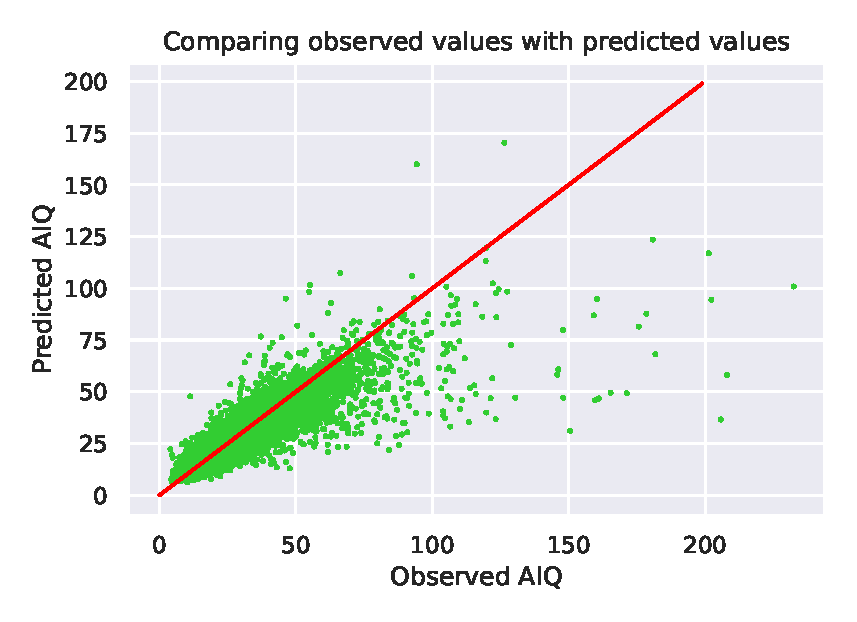
\includegraphics[width = 0.4\textwidth]{observed-vs-predicted-aiq.eps}
    \caption{Comparing the AQI calculated by observed pollutants and predicted. Points below the red line indicate underestimated predictions.}
    \label{fig:observed-vs-predicted-aqi}
\end{figure}

\begin{figure}
    \centering
    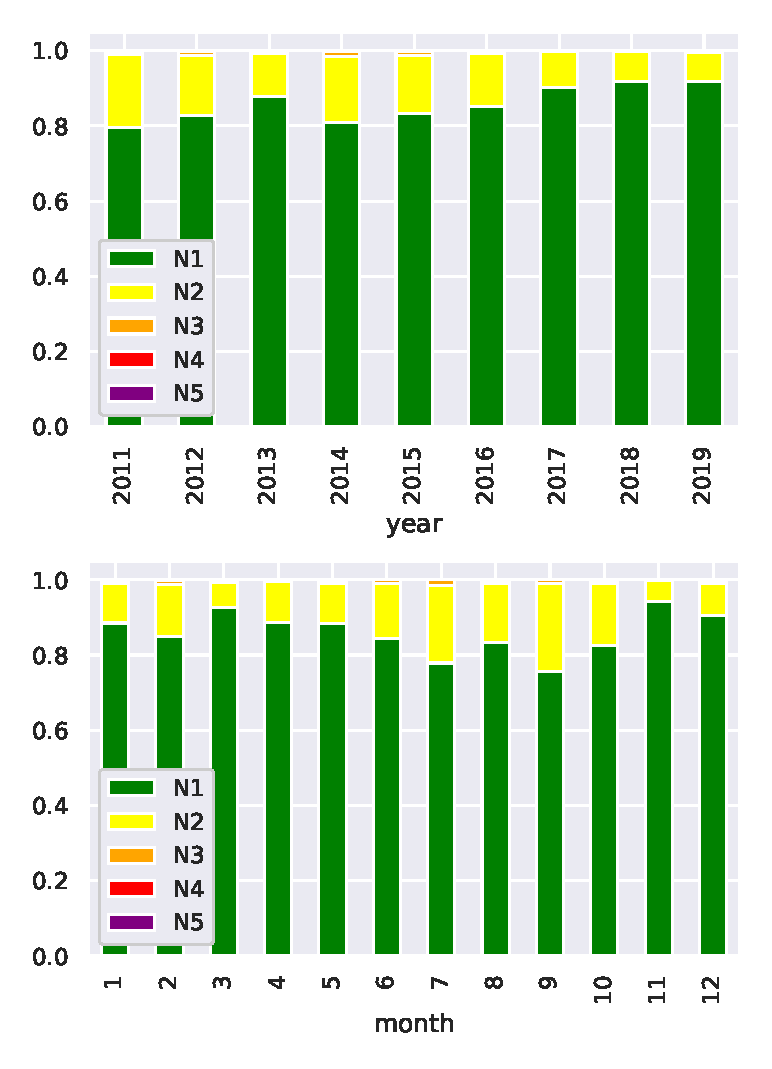
\includegraphics[width = 0.36\textwidth]{aiq-time.eps}
    \caption{Composition of AQI classes predicted in Tijuca: Year-based and Month-based.}
    \label{fig:aqitime}
\end{figure}

\begin{figure}
    \centering
    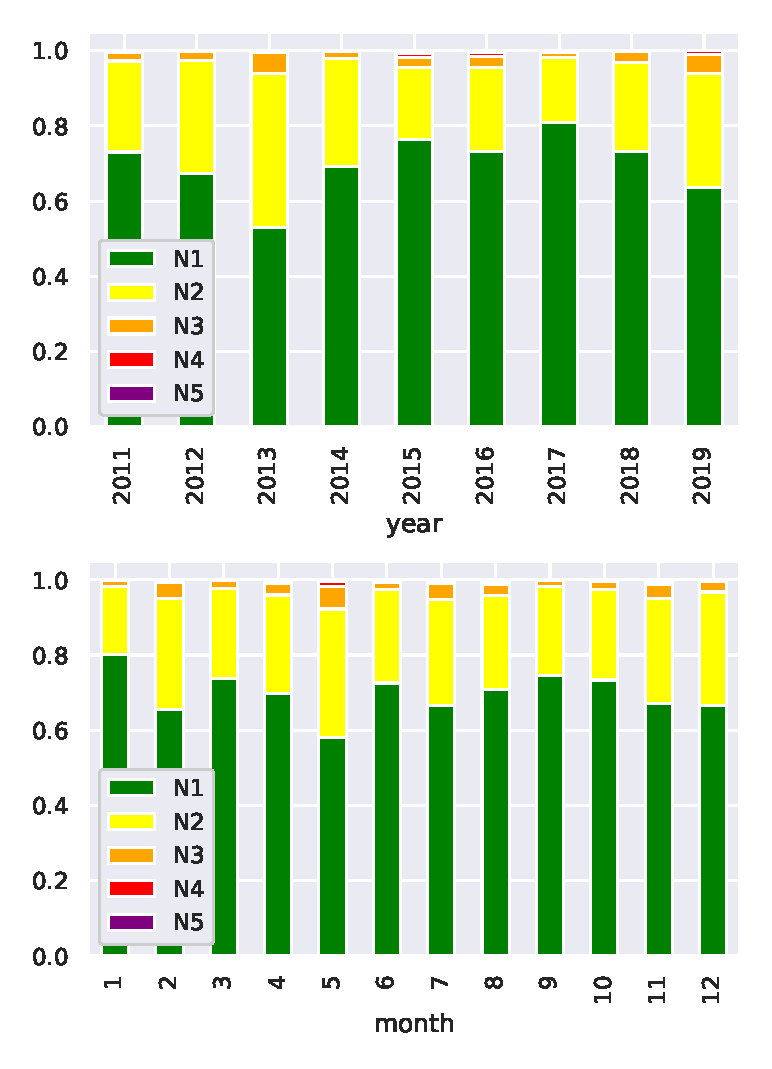
\includegraphics[width = 0.36\textwidth]{aiq-time-observed.eps}
    \caption{Composition of AQI classes observed in Tijuca: Year-based and Month-based.}
    \label{fig:aqitime-observed}
\end{figure}

\subsection{Aggregated results}

After studying the models with Tijuca station, we now apply to other stations
and report the results. The models tested will keep the same hyperparameters,
since the computation time would take too much longer. The considered models
are the three best for each pollutant. Table \ref{tab:summary-results}
sumarizes the results. The results for PM$_{10}$ in most cases showed the
best model for Tijuca is not for other locations. For CO and O$_3$ the results
had similar behavior. 

\begin{table*}
    \centering
    \resizebox{\textwidth}{!}{
        \begin{tabular}{|c|c|c|c|c|c|c|c|c|c|c|c|c|}
            \hline
         Gases  & \multicolumn{4}{c|}{\textbf{O$_3$}}                                & \multicolumn{4}{c|}{\textbf{CO}}                                 & \multicolumn{4}{c|}{\textbf{PM$_{10}$}}                                                                                        \\\hline
\textbf{Stations}           & \textbf{Method}   & \textbf{R$^2$} & \textbf{MAE} & \textbf{RMSE} & \textbf{Method} & \textbf{R$^2$} & \textbf{MAE} & \textbf{RMSE} & \textbf{Method}   & \textbf{R$^2$} & \textbf{MAE} & \textbf{RMSE} \\\hline
\multirow{3}{*}{\textbf{1}} & \textbf{SVR-RBF*} & 0.807          & 0.209        & 0.281         & \textbf{RF*}    & 0.668          & 0.248        & 0.367         & \textbf{RF}      & 0.771                              & 0.234                            & 0.315                             \\
            & \textbf{LR+EM*}   & 0.492          & 0.352        & 0.456         & \textbf{SVR-L*} & 0.643          & 0.257        & 0.381         & \textbf{SVR-L}   & 0.775                              & 0.233                            & 0.312                             \\
            & \textbf{SVR-L*}   & 0.816          & 0.202        & 0.274         & \textbf{LR+EM*} & 0.639          & 0.267        & 0.383         & \textbf{SVR-RBF*} & 0.769                              & 0.235                            & 0.316                             \\\hline
\multirow{3}{*}{\textbf{2}} & \textbf{SVR-RBF*} & 0.892          & 0.196        & 0.283         & \textbf{RF*}    & 0.770          & 0.251        & 0.350         & \textbf{RF}      & 0.777                              & 0.361                            & 0.493                             \\
            & \textbf{LR+EM*}   & 0.714          & 0.351        & 0.461         & \textbf{SVR-L*} & 0.777          & 0.244        & 0.345         & \textbf{SVR-L}   & 0.782                              & 0.353                            & 0.487                             \\
            & \textbf{SVR-L*}   & 0.881          & 0.207        & 0.297         & \textbf{LR+EM*} & 0.778          & 0.241        & 0.344         & \textbf{SVR-RBF*} & 0.766                              & 0.365                            & 0.505                             \\\hline
\multirow{3}{*}{\textbf{3}} & \textbf{SVR-RBF*} & 0.827          & 0.250        & 0.346         & \textbf{RF*}    & 0.861          & 0.216        & 0.298         & \textbf{RF}      & 0.761                              & 0.313                            & 0.411                             \\
            & \textbf{LR+EM*}   & 0.518          & 0.443        & 0.578         & \textbf{SVR-L*} & 0.860          & 0.215        & 0.299         & \textbf{SVR-L}   & 0.773                              & 0.305                            & 0.401                             \\
            & \textbf{SVR-L*}   & 0.832          & 0.248        & 0.341         & \textbf{LR+EM*} & 0.858          & 0.217        & 0.301         & \textbf{SVR-RBF*} & 0.746                              & 0.321                            & 0.425                             \\\hline
\multirow{3}{*}{\textbf{4}} & \textbf{SVR-RBF*} & 0.909          & 0.198        & 0.276         & \textbf{RF*}    & 0.833          & 0.235        & 0.324         & \textbf{RF}      & 0.757                              & 0.304                            & 0.413                             \\
            & \textbf{LR+EM*}   & 0.743          & 0.354        & 0.464         & \textbf{SVR-L*} & 0.826          & 0.235        & 0.331         & \textbf{SVR-L}   & 0.758                              & 0.300                            & 0.412                             \\
            & \textbf{SVR-L*}   & 0.900          & 0.210        & 0.290         & \textbf{LR+EM*} & 0.825          & 0.238        & 0.332         & \textbf{SVR-RBF*} & 0.742                              & 0.311                            & 0.425                             \\\hline
\multirow{3}{*}{\textbf{5}} & \textbf{SVR-RBF*} & 0.886          & 0.223        & 0.303         & \textbf{RF*}    & 0.800          & 0.253        & 0.347         & \textbf{RF}      & 0.781                              & 0.341                            & 0.451                             \\
            & \textbf{LR+EM*}   & 0.668          & 0.401        & 0.516         & \textbf{SVR-L*} & 0.790          & 0.257        & 0.356         & \textbf{SVR-L}   & 0.800                              & 0.321                            & 0.431                             \\
            & \textbf{SVR-L*}   & 0.884          & 0.224        & 0.305         & \textbf{LR+EM*} & 0.781          & 0.263        & 0.363         & \textbf{SVR-RBF*} & 0.769                              & 0.342                            & 0.463                             \\\hline
\multirow{3}{*}{\textbf{6}} & \textbf{SVR-RBF*} & 0.916          & 0.158        & 0.235         & \textbf{-}      & \textbf{-}     & \textbf{-}   & \textbf{-}    & \textbf{RF}      & 0.782                              & 0.357                            & 0.482                             \\
            & \textbf{LR+EM*}   & 0.755          & 0.297        & 0.401         & \textbf{-}      & \textbf{-}     & \textbf{-}   & \textbf{-}    & \textbf{SVR-L}   & 0.777                              & 0.362                            & 0.488                             \\
            & \textbf{SVR-L*}   & 0.911          & 0.160        & 0.242         & \textbf{-}      & \textbf{-}     & \textbf{-}   & \textbf{-}    & \textbf{SVR-RBF*} & 0.789                              & 0.351                            & 0.475                             \\\hline
\multirow{3}{*}{\textbf{7}} & \textbf{SVR-RBF*} & 0.868          & 0.270        & 0.371         & \textbf{RF*}    & 0.784          & 0.289        & 0.424         & \textbf{RF}      & 0.741                              & 0.362                            & 0.482                             \\
            & \textbf{LR+EM*}   & 0.655          & 0.456        & 0.599         & \textbf{SVR-L*} & 0.770          & 0.291        & 0.437         & \textbf{SVR-L}   & 0.751                              & 0.354                            & 0.474                             \\
            & \textbf{SVR-L*}   & 0.866          & 0.271        & 0.374
            & \textbf{LR+EM*} & 0.765          & 0.301        & 0.442
            & \textbf{SVR-RBF*} & 0.726                              & 0.370
            & 0.496 \\\hline
\end{tabular}
    }
    \caption{Summary results in the testing set for each station and each gas. LR = Linear Regression, SVR-L = SVR with linear kernel, RF = Random Forest, and * when best features are used.}
    \label{tab:summary-results}
\end{table*}

\section{Discussion and future work}
\label{sec:discussion}

All the models had a bad behavior of underestimate the pollutant values. One
possible way to handle this problem would be to weight error above and below
the observed differently. For instance, if the estimate is above the observed
value, the weight will be larger, and if is below, it will be smaller. Besides
that problem, the results were quite interesting, specially for ozone and
carbon monoxide. Particulate matter had the worst results in general, so other
endogenous variables should be considered. Other important consideration is
the computation time. Considering all the process, more than 12 hours of CPU
time running the Jupyter Notebooks, even with the simplifications. The
relation between the pollutants and the meteorological was overestimated by us
previously. It seems that the lag variables from the pollutants are very
important. Perhaps more specific functions of these variables should be
modeled. 

Some possible extensions and subproducts: 

\begin{enumerate}
    \item Daily predictions: here the daily predictions were not good and were
    disregarded; 
    \item Traffic car variable: other works showed the importance of this
    variable; 
    \item Prediction of non monitored locations: this is a subproduct of the
    models not explored. 
\end{enumerate}

\section{Conclusion}
\label{sec:conclusion}

Air quality forecast is a hard task as mentioned in Section
\ref{sec:polluting-gases} given the complex interactions. On the other hand,
the ability to estimate these quantities (or even control it!) is becoming
more important in urban areas since the impacts on the community and the
environment. This work presentes a study of some models to forecast
pollutants' levels and AQI. It produced a suitable hourly model with a
reasonable accuracy for each monitoring station in RIo de Janeiro.

\section{Code and data availability}

The data and code are open source. The data is available at
\cite{dataset-rio-ar-quality}, while the code are available at Github
repository\footnote{\url{https://github.com/lucasmoschen/machine-learning-project}}.
All the codes are separated by Jupyter Notebooks, describing all the steps:
EDA, Data Engineering, Models for O3, CO, PM10, and AIQ, and an Aggregated
model. 